% Publication figures for the ACFL journal manuscript.
% Regenerate: ./acfl_env/bin/python docs/manuscript/generate_figures.py

\begin{figure}[t]
\centering
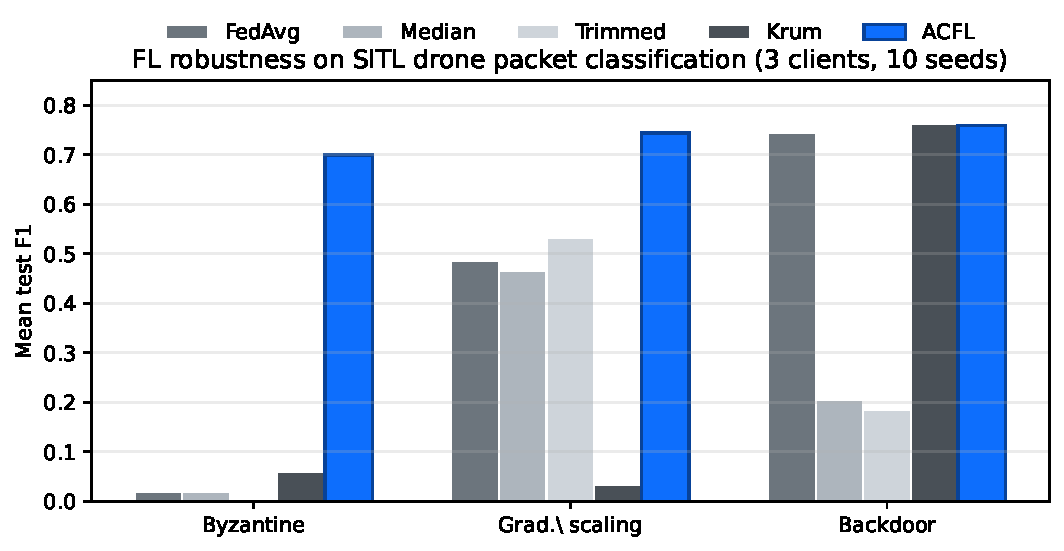
\includegraphics[width=\linewidth]{figures/fig_main_f1.pdf}
\caption{Mean test F1 across defenders and attacks on the SITL drone packet FL benchmark (3 clients, 12 rounds, 10 seeds). Only ACFL preserves utility under Byzantine attack; classical robust aggregators collapse or underperform FedAvg on gradient scaling and backdoor.}
\label{fig:main-f1}
\end{figure}

\begin{figure}[t]
\centering
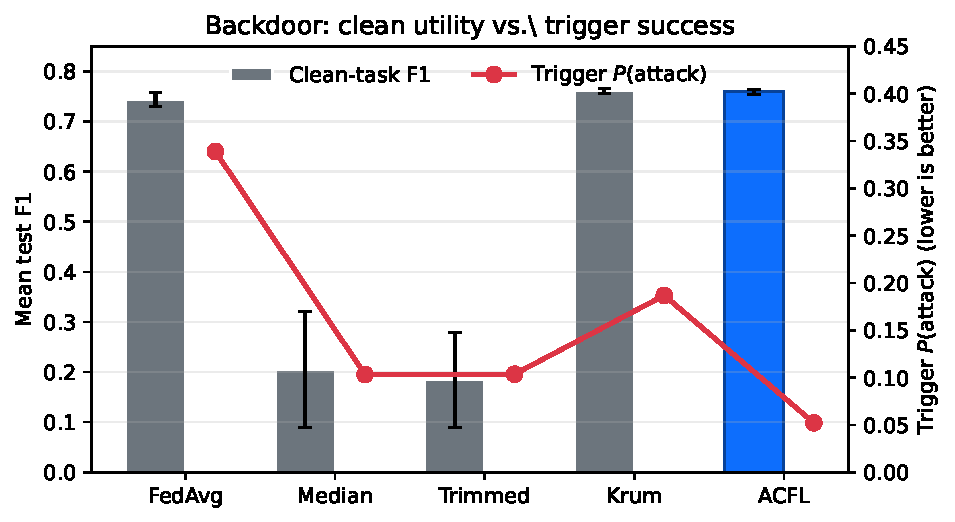
\includegraphics[width=\linewidth]{figures/fig_backdoor_dual.pdf}
\caption{Backdoor attack: clean-task F1 (bars, left axis) versus mean trigger $P(\text{attack})$ on counterfactual probes (line, right axis). Lower trigger probability indicates less successful backdoor activation. ACFL reduces trigger success relative to FedAvg and Krum while matching clean-task F1.}
\label{fig:backdoor-dual}
\end{figure}
